\documentclass[border=4pt]{standalone}
\usepackage{tikz}
\usepackage{pgfplots}
\pgfplotsset{compat=1.18}
\usetikzlibrary{shapes.geometric,arrows.meta,positioning,fit,calc,decorations.pathreplacing}
\usepackage{xcolor}
\definecolor{bestcol}{HTML}{1565C0}
\definecolor{freegreen}{HTML}{2E7D32}
\definecolor{learnblue}{HTML}{1565C0}
\definecolor{fusred}{HTML}{C62828}
\newcommand{\best}[1]{{\color{bestcol}\textbf{#1}}}
\begin{document}
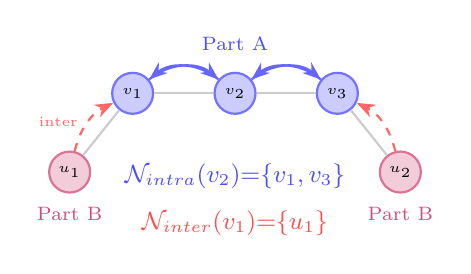
\begin{tikzpicture}[
  every node/.style={font=\scriptsize},
  jnt/.style={circle, draw, minimum size=0.52cm, inner sep=0pt,
              font=\tiny\bfseries, thick},
  blue jnt/.style={jnt, fill=blue!20, draw=blue!55},
  purp jnt/.style={jnt, fill=purple!20, draw=purple!55},
  sk/.style={gray!40, thick},
  intra/.style={-Stealth, blue!60, thick, bend left=40},
  inter/.style={-Stealth, red!60, thick, dashed, bend left=30}
]
%% Part A (e.g. arm, 3 joints)
\node[blue jnt] (v1) at (0, 0)   {$v_1$};
\node[blue jnt] (v2) at (1.3, 0) {$v_2$};
\node[blue jnt] (v3) at (2.6, 0) {$v_3$};
%% Part B boundary joints
\node[purp jnt] (u1) at (-0.8,-1.0) {$u_1$};
\node[purp jnt] (u2) at ( 3.4,-1.0) {$u_2$};

%% skeleton
\foreach \a/\b in {u1/v1, v1/v2, v2/v3, v3/u2}
  \draw[sk] (\a)--(\b);

%% intra arrows
\draw[intra] (v1) to (v2);
\draw[intra] (v2) to (v3);
\draw[intra, bend right=40] (v2) to (v1);
\draw[intra, bend right=40] (v3) to (v2);

%% inter arrows
\draw[inter, bend left=25]  (u1) to node[left,font=\tiny,text=red!60]{inter} (v1);
\draw[inter, bend right=25] (u2) to (v3);

%% labels below
\node[below=0.5cm of v2, text=blue!70, align=center]
  {\small$\mathcal{N}_{\text{intra}}(v_2){=}\{v_1,v_3\}$};
\node[below=1.1cm of v2, text=red!70, align=center]
  {\small$\mathcal{N}_{\text{inter}}(v_1){=}\{u_1\}$};

%% part labels
\node[above=0.15cm of v2, text=blue!70] {Part A};
\node[below=0.05cm of u1, text=purple!70] {Part B};
\node[below=0.05cm of u2, text=purple!70] {Part B};
\end{tikzpicture}
\end{document}
